\documentclass[dvipdfmx]{standalone}
\usepackage{tecfig}
\begin{document}
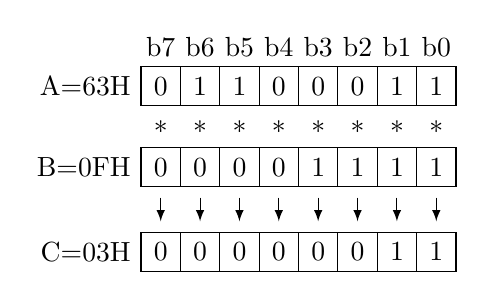
\begin{tikzpicture}[x=5mm, y=5mm]
	\tikzstyle{fixed}=[anchor=north, minimum width=5mm, minimum height=5mm]
		\foreach \x in {0,1,...,7}{
			\node (b\x) at (7-\x, 0) {b\x};
			\node[fixed, draw] (c\x) at (b\x.south) {};
			\node[fixed] (d\x) at (c\x.south) {$\ast$};
			\node[fixed, draw] (e\x) at (d\x.south) {};
			\node[fixed] (f\x) at (e\x.south) {\tikz \draw[-latex] (0, 0) -- (0, -3mm);};
			\node[fixed, draw] (g\x) at (f\x.south) {};
		}
		\foreach \y [count=\x from 0] in {1,1,0,0,0,1,1,0}
			\node at (c\x) {\y};
		\foreach \y [count=\x from 0] in {1,1,1,1,0,0,0,0}
			\node at (e\x) {\y};
		\foreach \y [count=\x from 0] in {1,1,0,0,0,0,0,0}
			\node at (g\x) {\y};
		\node[anchor=east, align=left] at (c7.west) {A=63H};
		\node[anchor=east, align=left] at (e7.west) {B=0FH};
		\node[anchor=east, align=left] at (g7.west) {C=03H};
	\end{tikzpicture}
\end{document}
